\documentclass[1p]{elsarticle_modified}
%\bibliographystyle{elsarticle-num}

%\usepackage[colorlinks]{hyperref}
%\usepackage{abbrmath_seonhwa} %\Abb, \Ascr, \Acal ,\Abf, \Afrak
\usepackage{amsfonts}
\usepackage{amssymb}
\usepackage{amsmath}
\usepackage{amsthm}
\usepackage{scalefnt}
\usepackage{amsbsy}
\usepackage{kotex}
\usepackage{caption}
\usepackage{subfig}
\usepackage{color}
\usepackage{graphicx}
\usepackage{xcolor} %% white, black, red, green, blue, cyan, magenta, yellow
\usepackage{float}
\usepackage{setspace}
\usepackage{hyperref}

\usepackage{tikz}
\usetikzlibrary{arrows}

\usepackage{multirow}
\usepackage{array} % fixed length table
\usepackage{hhline}

%%%%%%%%%%%%%%%%%%%%%
\makeatletter
\renewcommand*\env@matrix[1][\arraystretch]{%
	\edef\arraystretch{#1}%
	\hskip -\arraycolsep
	\let\@ifnextchar\new@ifnextchar
	\array{*\c@MaxMatrixCols c}}
\makeatother %https://tex.stackexchange.com/questions/14071/how-can-i-increase-the-line-spacing-in-a-matrix
%%%%%%%%%%%%%%%

\usepackage[normalem]{ulem}

\newcommand{\msout}[1]{\ifmmode\text{\sout{\ensuremath{#1}}}\else\sout{#1}\fi}
%SOURCE: \msout is \stkout macro in https://tex.stackexchange.com/questions/20609/strikeout-in-math-mode

\newcommand{\cancel}[1]{
	\ifmmode
	{\color{red}\msout{#1}}
	\else
	{\color{red}\sout{#1}}
	\fi
}

\newcommand{\add}[1]{
	{\color{blue}\uwave{#1}}
}

\newcommand{\replace}[2]{
	\ifmmode
	{\color{red}\msout{#1}}{\color{blue}\uwave{#2}}
	\else
	{\color{red}\sout{#1}}{\color{blue}\uwave{#2}}
	\fi
}

\newcommand{\Sol}{\mathcal{S}} %segment
\newcommand{\D}{D} %diagram
\newcommand{\A}{\mathcal{A}} %arc


%%%%%%%%%%%%%%%%%%%%%%%%%%%%%5 test

\def\sl{\operatorname{\textup{SL}}(2,\Cbb)}
\def\psl{\operatorname{\textup{PSL}}(2,\Cbb)}
\def\quan{\mkern 1mu \triangleright \mkern 1mu}

\theoremstyle{definition}
\newtheorem{thm}{Theorem}[section]
\newtheorem{prop}[thm]{Proposition}
\newtheorem{lem}[thm]{Lemma}
\newtheorem{ques}[thm]{Question}
\newtheorem{cor}[thm]{Corollary}
\newtheorem{defn}[thm]{Definition}
\newtheorem{exam}[thm]{Example}
\newtheorem{rmk}[thm]{Remark}
\newtheorem{alg}[thm]{Algorithm}

\newcommand{\I}{\sqrt{-1}}
\begin{document}

%\begin{frontmatter}
%
%\title{Boundary parabolic representations of knots up to 8 crossings}
%
%%% Group authors per affiliation:
%\author{Yunhi Cho} 
%\address{Department of Mathematics, University of Seoul, Seoul, Korea}
%\ead{yhcho@uos.ac.kr}
%
%
%\author{Seonhwa Kim} %\fnref{s_kim}}
%\address{Center for Geometry and Physics, Institute for Basic Science, Pohang, 37673, Korea}
%\ead{ryeona17@ibs.re.kr}
%
%\author{Hyuk Kim}
%\address{Department of Mathematical Sciences, Seoul National University, Seoul 08826, Korea}
%\ead{hyukkim@snu.ac.kr}
%
%\author{Seokbeom Yoon}
%\address{Department of Mathematical Sciences, Seoul National University, Seoul, 08826,  Korea}
%\ead{sbyoon15@snu.ac.kr}
%
%\begin{abstract}
%We find all boundary parabolic representation of knots up to 8 crossings.
%
%\end{abstract}
%\begin{keyword}
%    \MSC[2010] 57M25 
%\end{keyword}
%
%\end{frontmatter}

%\linenumbers
%\tableofcontents
%
\newcommand\colored[1]{\textcolor{white}{\rule[-0.35ex]{0.8em}{1.4ex}}\kern-0.8em\color{red} #1}%
%\newcommand\colored[1]{\textcolor{white}{ #1}\kern-2.17ex	\textcolor{white}{ #1}\kern-1.81ex	\textcolor{white}{ #1}\kern-2.15ex\color{red}#1	}

{\Large $\underline{12a_{1272}~(K12a_{1272})}$}

\setlength{\tabcolsep}{10pt}
\renewcommand{\arraystretch}{1.6}
\vspace{1cm}\begin{tabular}{m{100pt}>{\centering\arraybackslash}m{274pt}}
\multirow{5}{120pt}{
	\centering
	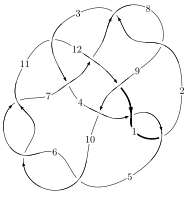
\includegraphics[width=112pt]{../../../GIT/diagram.site/Diagrams/png/2073_12a_1272.png}\\
\ \ \ A knot diagram\footnotemark}&
\allowdisplaybreaks
\textbf{Linearized knot diagam} \\
\cline{2-2}
 &
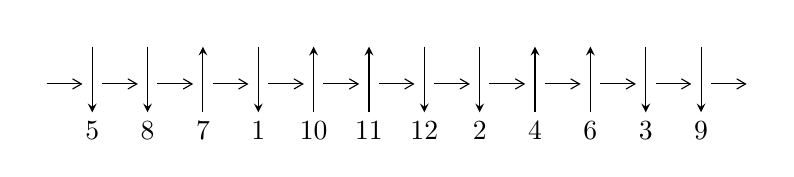
\begin{tikzpicture}[x=20pt, y=17pt]
	% nodes
	\node (C0) at (0, 0) {};
	\node (C1) at (1, 0) {};
	\node (C1U) at (1, +1) {};
	\node (C1D) at (1, -1) {5};

	\node (C2) at (2, 0) {};
	\node (C2U) at (2, +1) {};
	\node (C2D) at (2, -1) {8};

	\node (C3) at (3, 0) {};
	\node (C3U) at (3, +1) {};
	\node (C3D) at (3, -1) {7};

	\node (C4) at (4, 0) {};
	\node (C4U) at (4, +1) {};
	\node (C4D) at (4, -1) {1};

	\node (C5) at (5, 0) {};
	\node (C5U) at (5, +1) {};
	\node (C5D) at (5, -1) {10};

	\node (C6) at (6, 0) {};
	\node (C6U) at (6, +1) {};
	\node (C6D) at (6, -1) {11};

	\node (C7) at (7, 0) {};
	\node (C7U) at (7, +1) {};
	\node (C7D) at (7, -1) {12};

	\node (C8) at (8, 0) {};
	\node (C8U) at (8, +1) {};
	\node (C8D) at (8, -1) {2};

	\node (C9) at (9, 0) {};
	\node (C9U) at (9, +1) {};
	\node (C9D) at (9, -1) {4};

	\node (C10) at (10, 0) {};
	\node (C10U) at (10, +1) {};
	\node (C10D) at (10, -1) {6};

	\node (C11) at (11, 0) {};
	\node (C11U) at (11, +1) {};
	\node (C11D) at (11, -1) {3};

	\node (C12) at (12, 0) {};
	\node (C12U) at (12, +1) {};
	\node (C12D) at (12, -1) {9};
	\node (C13) at (13, 0) {};

	% arrows
	\draw[->,>={angle 60}]
	(C0) edge (C1) (C1) edge (C2) (C2) edge (C3) (C3) edge (C4) (C4) edge (C5) (C5) edge (C6) (C6) edge (C7) (C7) edge (C8) (C8) edge (C9) (C9) edge (C10) (C10) edge (C11) (C11) edge (C12) (C12) edge (C13) ;	\draw[->,>=stealth]
	(C1U) edge (C1D) (C2U) edge (C2D) (C3D) edge (C3U) (C4U) edge (C4D) (C5D) edge (C5U) (C6D) edge (C6U) (C7U) edge (C7D) (C8U) edge (C8D) (C9D) edge (C9U) (C10D) edge (C10U) (C11U) edge (C11D) (C12U) edge (C12D) ;
	\end{tikzpicture} \\
\hhline{~~} \\& 
\textbf{Solving Sequence} \\ \cline{2-2} 
 &
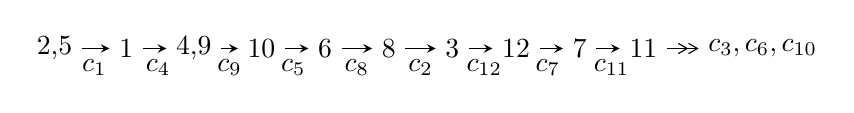
\begin{tikzpicture}[x=23pt, y=7pt]
	% node
	\node (A0) at (-1/8, 0) {2,5};
	\node (A1) at (1, 0) {1};
	\node (A2) at (33/16, 0) {4,9};
	\node (A3) at (25/8, 0) {10};
	\node (A4) at (33/8, 0) {6};
	\node (A5) at (41/8, 0) {8};
	\node (A6) at (49/8, 0) {3};
	\node (A7) at (57/8, 0) {12};
	\node (A8) at (65/8, 0) {7};
	\node (A9) at (73/8, 0) {11};
	\node (C1) at (1/2, -1) {$c_{1}$};
	\node (C2) at (3/2, -1) {$c_{4}$};
	\node (C3) at (21/8, -1) {$c_{9}$};
	\node (C4) at (29/8, -1) {$c_{5}$};
	\node (C5) at (37/8, -1) {$c_{8}$};
	\node (C6) at (45/8, -1) {$c_{2}$};
	\node (C7) at (53/8, -1) {$c_{12}$};
	\node (C8) at (61/8, -1) {$c_{7}$};
	\node (C9) at (69/8, -1) {$c_{11}$};
	\node (A10) at (11, 0) {$c_{3},c_{6},c_{10}$};

	% edge
	\draw[->,>=stealth]	
	(A0) edge (A1) (A1) edge (A2) (A2) edge (A3) (A3) edge (A4) (A4) edge (A5) (A5) edge (A6) (A6) edge (A7) (A7) edge (A8) (A8) edge (A9) ;
	\draw[->>,>={angle 60}]	
	(A9) edge (A10);
\end{tikzpicture} \\ 

\end{tabular} \\

\footnotetext{
The image of knot diagram is generated by the software ``\textbf{Draw programme}" developed by Andrew Bartholomew(\url{http://www.layer8.co.uk/maths/draw/index.htm\#Running-draw}), where we modified some parts for our purpose(\url{https://github.com/CATsTAILs/LinksPainter}).
}\phantom \\ \newline 
\centering \textbf{Ideals for irreducible components\footnotemark of $X_{\text{par}}$} 
 
\begin{align*}
I^u_{1}&=\langle 
-5.27398\times10^{429} u^{131}-9.58434\times10^{429} u^{130}+\cdots+9.61277\times10^{428} b-5.45766\times10^{432},\\
\phantom{I^u_{1}}&\phantom{= \langle  }1.80780\times10^{432} u^{131}+3.29725\times10^{432} u^{130}+\cdots+2.02829\times10^{431} a+1.86013\times10^{435},\\
\phantom{I^u_{1}}&\phantom{= \langle  }u^{132}+u^{131}+\cdots-1451 u-844\rangle \\
I^u_{2}&=\langle 
2318651091 u^{29}+8025321455 u^{28}+\cdots+9372903 b+4797253946,\\
\phantom{I^u_{2}}&\phantom{= \langle  }-1257579720 u^{29}-4274580356 u^{28}+\cdots+9372903 a-2710745983,\;u^{30}+4 u^{29}+\cdots+7 u+1\rangle \\
I^u_{3}&=\langle 
b+a-1,\;a^2-3 a+3,\;u-1\rangle \\
\\
\end{align*}
\raggedright * 3 irreducible components of $\dim_{\mathbb{C}}=0$, with total 164 representations.\\
\footnotetext{All coefficients of polynomials are rational numbers. But the coefficients are sometimes approximated in decimal forms when there is not enough margin.}
\newpage
\renewcommand{\arraystretch}{1}
\centering \section*{I. $I^u_{1}= \langle -5.27\times10^{429} u^{131}-9.58\times10^{429} u^{130}+\cdots+9.61\times10^{428} b-5.46\times10^{432},\;1.81\times10^{432} u^{131}+3.30\times10^{432} u^{130}+\cdots+2.03\times10^{431} a+1.86\times10^{435},\;u^{132}+u^{131}+\cdots-1451 u-844 \rangle$}
\flushleft \textbf{(i) Arc colorings}\\
\begin{tabular}{m{7pt} m{180pt} m{7pt} m{180pt} }
\flushright $a_{2}=$&$\begin{pmatrix}1\\0\end{pmatrix}$ \\
\flushright $a_{5}=$&$\begin{pmatrix}0\\u\end{pmatrix}$ \\
\flushright $a_{1}=$&$\begin{pmatrix}1\\- u^2\end{pmatrix}$ \\
\flushright $a_{4}=$&$\begin{pmatrix}u\\- u^3+u\end{pmatrix}$ \\
\flushright $a_{9}=$&$\begin{pmatrix}-8.91293 u^{131}-16.2563 u^{130}+\cdots-26935.2 u-9170.89\\5.48643 u^{131}+9.97042 u^{130}+\cdots+16692.0 u+5677.51\end{pmatrix}$ \\
\flushright $a_{10}=$&$\begin{pmatrix}-3.34622 u^{131}-6.13050 u^{130}+\cdots-9951.53 u-3393.85\\7.33783 u^{131}+13.3479 u^{130}+\cdots+22362.1 u+7606.69\end{pmatrix}$ \\
\flushright $a_{6}=$&$\begin{pmatrix}-4.96312 u^{131}-9.02635 u^{130}+\cdots-15167.5 u-5149.06\\12.2350 u^{131}+22.1179 u^{130}+\cdots+37446.3 u+12681.3\end{pmatrix}$ \\
\flushright $a_{8}=$&$\begin{pmatrix}-3.42650 u^{131}-6.28584 u^{130}+\cdots-10243.3 u-3493.38\\5.48643 u^{131}+9.97042 u^{130}+\cdots+16692.0 u+5677.51\end{pmatrix}$ \\
\flushright $a_{3}=$&$\begin{pmatrix}11.5848 u^{131}+21.0113 u^{130}+\cdots+35412.9 u+12022.8\\-19.5383 u^{131}-35.3500 u^{130}+\cdots-60023.3 u-20340.8\end{pmatrix}$ \\
\flushright $a_{12}=$&$\begin{pmatrix}0.967020 u^{131}+1.73517 u^{130}+\cdots+3148.59 u+1041.78\\-0.912310 u^{131}-1.60702 u^{130}+\cdots-2865.28 u-960.299\end{pmatrix}$ \\
\flushright $a_{7}=$&$\begin{pmatrix}-4.07589 u^{131}-7.57566 u^{130}+\cdots-11810.1 u-4058.04\\6.06028 u^{131}+10.9765 u^{130}+\cdots+18294.1 u+6226.53\end{pmatrix}$ \\
\flushright $a_{11}=$&$\begin{pmatrix}5.61423 u^{131}+10.2551 u^{130}+\cdots+16930.8 u+5749.34\\-11.4857 u^{131}-20.7801 u^{130}+\cdots-35554.7 u-12041.1\end{pmatrix}$\\&\end{tabular}
\flushleft \textbf{(ii) Obstruction class $= -1$}\\~\\
\flushleft \textbf{(iii) Cusp Shapes $= 769.616 u^{131}+1391.64 u^{130}+\cdots+2.37325\times10^{6} u+803188.$}\\~\\
\newpage\renewcommand{\arraystretch}{1}
\flushleft \textbf{(iv) u-Polynomials at the component}\newline \\
\begin{tabular}{m{50pt}|m{274pt}}
Crossings & \hspace{64pt}u-Polynomials at each crossing \\
\hline $$\begin{aligned}c_{1},c_{4}\end{aligned}$$&$\begin{aligned}
&u^{132}- u^{131}+\cdots+1451 u-844
\end{aligned}$\\
\hline $$\begin{aligned}c_{2},c_{8}\end{aligned}$$&$\begin{aligned}
&u^{132}+44 u^{130}+\cdots-21827 u-1189
\end{aligned}$\\
\hline $$\begin{aligned}c_{3}\end{aligned}$$&$\begin{aligned}
&u^{132}-4 u^{131}+\cdots+9472 u-2239
\end{aligned}$\\
\hline $$\begin{aligned}c_{5},c_{6},c_{10}\end{aligned}$$&$\begin{aligned}
&u^{132}+2 u^{131}+\cdots+130 u+19
\end{aligned}$\\
\hline $$\begin{aligned}c_{7}\end{aligned}$$&$\begin{aligned}
&u^{132}+u^{130}+\cdots-28 u+8
\end{aligned}$\\
\hline $$\begin{aligned}c_{9}\end{aligned}$$&$\begin{aligned}
&u^{132}-4 u^{130}+\cdots-37881 u+2437
\end{aligned}$\\
\hline $$\begin{aligned}c_{11}\end{aligned}$$&$\begin{aligned}
&u^{132}+6 u^{131}+\cdots+89459 u+56393
\end{aligned}$\\
\hline $$\begin{aligned}c_{12}\end{aligned}$$&$\begin{aligned}
&u^{132}-5 u^{131}+\cdots+4452 u+103
\end{aligned}$\\
\hline
\end{tabular}\\~\\
\newpage\renewcommand{\arraystretch}{1}
\flushleft \textbf{(v) Riley Polynomials at the component}\newline \\
\begin{tabular}{m{50pt}|m{274pt}}
Crossings & \hspace{64pt}Riley Polynomials at each crossing \\
\hline $$\begin{aligned}c_{1},c_{4}\end{aligned}$$&$\begin{aligned}
&y^{132}-63 y^{131}+\cdots-11311753 y+712336
\end{aligned}$\\
\hline $$\begin{aligned}c_{2},c_{8}\end{aligned}$$&$\begin{aligned}
&y^{132}+88 y^{131}+\cdots-71456419 y+1413721
\end{aligned}$\\
\hline $$\begin{aligned}c_{3}\end{aligned}$$&$\begin{aligned}
&y^{132}-36 y^{131}+\cdots-304367236 y+5013121
\end{aligned}$\\
\hline $$\begin{aligned}c_{5},c_{6},c_{10}\end{aligned}$$&$\begin{aligned}
&y^{132}-144 y^{131}+\cdots-14848 y+361
\end{aligned}$\\
\hline $$\begin{aligned}c_{7}\end{aligned}$$&$\begin{aligned}
&y^{132}+2 y^{131}+\cdots-4464 y+64
\end{aligned}$\\
\hline $$\begin{aligned}c_{9}\end{aligned}$$&$\begin{aligned}
&y^{132}-8 y^{131}+\cdots-75967363 y+5938969
\end{aligned}$\\
\hline $$\begin{aligned}c_{11}\end{aligned}$$&$\begin{aligned}
&y^{132}+62 y^{131}+\cdots+237776842153 y+3180170449
\end{aligned}$\\
\hline $$\begin{aligned}c_{12}\end{aligned}$$&$\begin{aligned}
&y^{132}-27 y^{131}+\cdots-6883504 y+10609
\end{aligned}$\\
\hline
\end{tabular}\\~\\
\newpage\flushleft \textbf{(vi) Complex Volumes and Cusp Shapes}
$$\begin{array}{c|c|c}  
\text{Solutions to }I^u_{1}& \I (\text{vol} + \sqrt{-1}CS) & \text{Cusp shape}\\
 \hline 
\begin{aligned}
u &= \phantom{-}0.888433 + 0.459649 I \\
a &= -0.192013 + 1.130340 I \\
b &= \phantom{-}0.135369 + 1.366530 I\end{aligned}
 & \phantom{-}10.08520 - 8.84662 I & \phantom{-0.000000 } 0 \\ \hline\begin{aligned}
u &= \phantom{-}0.888433 - 0.459649 I \\
a &= -0.192013 - 1.130340 I \\
b &= \phantom{-}0.135369 - 1.366530 I\end{aligned}
 & \phantom{-}10.08520 + 8.84662 I & \phantom{-0.000000 } 0 \\ \hline\begin{aligned}
u &= -0.860001 + 0.505931 I \\
a &= -0.524831 - 0.211304 I \\
b &= \phantom{-}0.00912 - 1.53664 I\end{aligned}
 & \phantom{-}10.41720 + 2.03214 I & \phantom{-0.000000 } 0 \\ \hline\begin{aligned}
u &= -0.860001 - 0.505931 I \\
a &= -0.524831 + 0.211304 I \\
b &= \phantom{-}0.00912 + 1.53664 I\end{aligned}
 & \phantom{-}10.41720 - 2.03214 I & \phantom{-0.000000 } 0 \\ \hline\begin{aligned}
u &= -0.128893 + 0.987034 I \\
a &= -0.107867 + 0.455133 I \\
b &= -1.064690 - 0.044525 I\end{aligned}
 & \phantom{-}6.25496 - 6.63131 I & \phantom{-0.000000 } 0 \\ \hline\begin{aligned}
u &= -0.128893 - 0.987034 I \\
a &= -0.107867 - 0.455133 I \\
b &= -1.064690 + 0.044525 I\end{aligned}
 & \phantom{-}6.25496 + 6.63131 I & \phantom{-0.000000 } 0 \\ \hline\begin{aligned}
u &= -0.817665 + 0.595071 I \\
a &= -1.375280 - 0.085348 I \\
b &= -0.01154 - 1.61726 I\end{aligned}
 & \phantom{-}10.91990 + 2.34128 I & \phantom{-0.000000 } 0 \\ \hline\begin{aligned}
u &= -0.817665 - 0.595071 I \\
a &= -1.375280 + 0.085348 I \\
b &= -0.01154 + 1.61726 I\end{aligned}
 & \phantom{-}10.91990 - 2.34128 I & \phantom{-0.000000 } 0 \\ \hline\begin{aligned}
u &= -0.887029 + 0.426126 I \\
a &= -0.238037 - 0.107971 I \\
b &= \phantom{-}0.44793 + 1.51254 I\end{aligned}
 & \phantom{-}9.85464 - 4.57208 I & \phantom{-0.000000 } 0 \\ \hline\begin{aligned}
u &= -0.887029 - 0.426126 I \\
a &= -0.238037 + 0.107971 I \\
b &= \phantom{-}0.44793 - 1.51254 I\end{aligned}
 & \phantom{-}9.85464 + 4.57208 I & \phantom{-0.000000 } 0\\
 \hline 
 \end{array}$$\newpage$$\begin{array}{c|c|c}  
\text{Solutions to }I^u_{1}& \I (\text{vol} + \sqrt{-1}CS) & \text{Cusp shape}\\
 \hline 
\begin{aligned}
u &= -0.299028 + 0.934814 I \\
a &= -0.339354 + 0.092362 I \\
b &= \phantom{-}0.388248 + 1.036060 I\end{aligned}
 & \phantom{-}6.49844 - 4.55251 I & \phantom{-0.000000 } 0 \\ \hline\begin{aligned}
u &= -0.299028 - 0.934814 I \\
a &= -0.339354 - 0.092362 I \\
b &= \phantom{-}0.388248 - 1.036060 I\end{aligned}
 & \phantom{-}6.49844 + 4.55251 I & \phantom{-0.000000 } 0 \\ \hline\begin{aligned}
u &= \phantom{-}0.259667 + 1.010660 I \\
a &= -0.136638 - 0.521034 I \\
b &= \phantom{-}0.403078 - 1.345030 I\end{aligned}
 & \phantom{-}3.78458 + 8.55429 I & \phantom{-0.000000 } 0 \\ \hline\begin{aligned}
u &= \phantom{-}0.259667 - 1.010660 I \\
a &= -0.136638 + 0.521034 I \\
b &= \phantom{-}0.403078 + 1.345030 I\end{aligned}
 & \phantom{-}3.78458 - 8.55429 I & \phantom{-0.000000 } 0 \\ \hline\begin{aligned}
u &= \phantom{-}0.881749 + 0.328399 I \\
a &= \phantom{-}2.48900 + 0.26366 I \\
b &= -0.17445 - 1.63310 I\end{aligned}
 & \phantom{-}9.18224 - 1.20024 I & \phantom{-0.000000 } 0 \\ \hline\begin{aligned}
u &= \phantom{-}0.881749 - 0.328399 I \\
a &= \phantom{-}2.48900 - 0.26366 I \\
b &= -0.17445 + 1.63310 I\end{aligned}
 & \phantom{-}9.18224 + 1.20024 I & \phantom{-0.000000 } 0 \\ \hline\begin{aligned}
u &= -0.971761 + 0.434578 I \\
a &= \phantom{-}1.40070 + 0.56574 I \\
b &= -0.282247 + 0.929840 I\end{aligned}
 & \phantom{-}1.49064 + 1.85110 I & \phantom{-0.000000 } 0 \\ \hline\begin{aligned}
u &= -0.971761 - 0.434578 I \\
a &= \phantom{-}1.40070 - 0.56574 I \\
b &= -0.282247 - 0.929840 I\end{aligned}
 & \phantom{-}1.49064 - 1.85110 I & \phantom{-0.000000 } 0 \\ \hline\begin{aligned}
u &= -0.917872 + 0.166230 I \\
a &= \phantom{-}1.326400 + 0.401788 I \\
b &= -0.149482 + 0.636067 I\end{aligned}
 & \phantom{-}1.40547 + 1.62272 I & \phantom{-0.000000 } 0 \\ \hline\begin{aligned}
u &= -0.917872 - 0.166230 I \\
a &= \phantom{-}1.326400 - 0.401788 I \\
b &= -0.149482 - 0.636067 I\end{aligned}
 & \phantom{-}1.40547 - 1.62272 I & \phantom{-0.000000 } 0\\
 \hline 
 \end{array}$$\newpage$$\begin{array}{c|c|c}  
\text{Solutions to }I^u_{1}& \I (\text{vol} + \sqrt{-1}CS) & \text{Cusp shape}\\
 \hline 
\begin{aligned}
u &= \phantom{-}0.902863 + 0.202398 I \\
a &= \phantom{-}1.93367 - 1.39062 I \\
b &= -0.181766 + 0.639474 I\end{aligned}
 & -0.956671 - 0.870714 I & \phantom{-0.000000 } 0 \\ \hline\begin{aligned}
u &= \phantom{-}0.902863 - 0.202398 I \\
a &= \phantom{-}1.93367 + 1.39062 I \\
b &= -0.181766 - 0.639474 I\end{aligned}
 & -0.956671 + 0.870714 I & \phantom{-0.000000 } 0 \\ \hline\begin{aligned}
u &= \phantom{-}0.924821\phantom{ +0.000000I} \\
a &= -3.20484\phantom{ +0.000000I} \\
b &= \phantom{-}2.41225\phantom{ +0.000000I}\end{aligned}
 & -0.379463\phantom{ +0.000000I} & \phantom{-0.000000 } 0 \\ \hline\begin{aligned}
u &= \phantom{-}0.919150 + 0.062875 I \\
a &= -1.22487 - 1.47381 I \\
b &= \phantom{-}0.43120 + 1.81191 I\end{aligned}
 & -0.312377 - 0.392334 I & \phantom{-0.000000 } 0 \\ \hline\begin{aligned}
u &= \phantom{-}0.919150 - 0.062875 I \\
a &= -1.22487 + 1.47381 I \\
b &= \phantom{-}0.43120 - 1.81191 I\end{aligned}
 & -0.312377 + 0.392334 I & \phantom{-0.000000 } 0 \\ \hline\begin{aligned}
u &= \phantom{-}0.854419 + 0.330939 I \\
a &= \phantom{-}1.40388 - 0.54442 I \\
b &= \phantom{-}0.05937 - 1.64090 I\end{aligned}
 & \phantom{-}9.26391 - 1.67107 I & \phantom{-0.000000 } 0 \\ \hline\begin{aligned}
u &= \phantom{-}0.854419 - 0.330939 I \\
a &= \phantom{-}1.40388 + 0.54442 I \\
b &= \phantom{-}0.05937 + 1.64090 I\end{aligned}
 & \phantom{-}9.26391 + 1.67107 I & \phantom{-0.000000 } 0 \\ \hline\begin{aligned}
u &= -0.747724 + 0.524870 I \\
a &= -2.12221 - 0.04445 I \\
b &= -0.080811 - 1.350620 I\end{aligned}
 & \phantom{-}10.74310 + 2.15226 I & \phantom{-0.000000 } 0 \\ \hline\begin{aligned}
u &= -0.747724 - 0.524870 I \\
a &= -2.12221 + 0.04445 I \\
b &= -0.080811 + 1.350620 I\end{aligned}
 & \phantom{-}10.74310 - 2.15226 I & \phantom{-0.000000 } 0 \\ \hline\begin{aligned}
u &= -0.989013 + 0.458677 I \\
a &= \phantom{-}2.20619 + 0.31109 I \\
b &= -0.232381 + 1.160650 I\end{aligned}
 & \phantom{-}1.20534 + 2.58602 I & \phantom{-0.000000 } 0\\
 \hline 
 \end{array}$$\newpage$$\begin{array}{c|c|c}  
\text{Solutions to }I^u_{1}& \I (\text{vol} + \sqrt{-1}CS) & \text{Cusp shape}\\
 \hline 
\begin{aligned}
u &= -0.989013 - 0.458677 I \\
a &= \phantom{-}2.20619 - 0.31109 I \\
b &= -0.232381 - 1.160650 I\end{aligned}
 & \phantom{-}1.20534 - 2.58602 I & \phantom{-0.000000 } 0 \\ \hline\begin{aligned}
u &= \phantom{-}1.017390 + 0.399155 I \\
a &= \phantom{-}2.00809 + 0.70527 I \\
b &= -0.011529 - 1.090260 I\end{aligned}
 & \phantom{-}2.53408 + 1.30747 I & \phantom{-0.000000 } 0 \\ \hline\begin{aligned}
u &= \phantom{-}1.017390 - 0.399155 I \\
a &= \phantom{-}2.00809 - 0.70527 I \\
b &= -0.011529 + 1.090260 I\end{aligned}
 & \phantom{-}2.53408 - 1.30747 I & \phantom{-0.000000 } 0 \\ \hline\begin{aligned}
u &= \phantom{-}1.025520 + 0.398648 I \\
a &= -1.23586 + 0.83864 I \\
b &= \phantom{-}0.657096 - 0.430489 I\end{aligned}
 & -3.47015 - 2.63906 I & \phantom{-0.000000 } 0 \\ \hline\begin{aligned}
u &= \phantom{-}1.025520 - 0.398648 I \\
a &= -1.23586 - 0.83864 I \\
b &= \phantom{-}0.657096 + 0.430489 I\end{aligned}
 & -3.47015 + 2.63906 I & \phantom{-0.000000 } 0 \\ \hline\begin{aligned}
u &= \phantom{-}0.777156 + 0.445739 I \\
a &= -2.98626 - 0.24164 I \\
b &= -0.139684 + 1.116770 I\end{aligned}
 & \phantom{-}10.45930 + 5.07607 I & \phantom{-0.000000 } 0 \\ \hline\begin{aligned}
u &= \phantom{-}0.777156 - 0.445739 I \\
a &= -2.98626 + 0.24164 I \\
b &= -0.139684 - 1.116770 I\end{aligned}
 & \phantom{-}10.45930 - 5.07607 I & \phantom{-0.000000 } 0 \\ \hline\begin{aligned}
u &= \phantom{-}1.086330 + 0.215183 I \\
a &= \phantom{-}1.114480 - 0.586549 I \\
b &= -1.144630 + 0.562319 I\end{aligned}
 & -1.66184 - 0.75099 I & \phantom{-0.000000 } 0 \\ \hline\begin{aligned}
u &= \phantom{-}1.086330 - 0.215183 I \\
a &= \phantom{-}1.114480 + 0.586549 I \\
b &= -1.144630 - 0.562319 I\end{aligned}
 & -1.66184 + 0.75099 I & \phantom{-0.000000 } 0 \\ \hline\begin{aligned}
u &= -0.798505 + 0.397196 I \\
a &= \phantom{-}2.86222 - 0.71894 I \\
b &= -0.63968 + 1.32038 I\end{aligned}
 & \phantom{-}10.17010 + 8.06121 I & \phantom{-0.000000 } 0\\
 \hline 
 \end{array}$$\newpage$$\begin{array}{c|c|c}  
\text{Solutions to }I^u_{1}& \I (\text{vol} + \sqrt{-1}CS) & \text{Cusp shape}\\
 \hline 
\begin{aligned}
u &= -0.798505 - 0.397196 I \\
a &= \phantom{-}2.86222 + 0.71894 I \\
b &= -0.63968 - 1.32038 I\end{aligned}
 & \phantom{-}10.17010 - 8.06121 I & \phantom{-0.000000 } 0 \\ \hline\begin{aligned}
u &= -1.065870 + 0.319329 I \\
a &= -0.671097 + 0.337438 I \\
b &= \phantom{-}0.065196 + 0.246846 I\end{aligned}
 & -1.06962 + 3.70198 I & \phantom{-0.000000 } 0 \\ \hline\begin{aligned}
u &= -1.065870 - 0.319329 I \\
a &= -0.671097 - 0.337438 I \\
b &= \phantom{-}0.065196 - 0.246846 I\end{aligned}
 & -1.06962 - 3.70198 I & \phantom{-0.000000 } 0 \\ \hline\begin{aligned}
u &= -1.045210 + 0.408453 I \\
a &= -1.81053 + 0.50219 I \\
b &= \phantom{-}0.63280 - 1.27162 I\end{aligned}
 & \phantom{-}2.58381 + 7.13715 I & \phantom{-0.000000 } 0 \\ \hline\begin{aligned}
u &= -1.045210 - 0.408453 I \\
a &= -1.81053 - 0.50219 I \\
b &= \phantom{-}0.63280 + 1.27162 I\end{aligned}
 & \phantom{-}2.58381 - 7.13715 I & \phantom{-0.000000 } 0 \\ \hline\begin{aligned}
u &= -0.159394 + 0.861713 I \\
a &= -0.568599 - 0.640734 I \\
b &= -0.457630 + 0.026165 I\end{aligned}
 & \phantom{-}7.95380 - 2.88865 I & \phantom{-0.000000 } 0 \\ \hline\begin{aligned}
u &= -0.159394 - 0.861713 I \\
a &= -0.568599 + 0.640734 I \\
b &= -0.457630 - 0.026165 I\end{aligned}
 & \phantom{-}7.95380 + 2.88865 I & \phantom{-0.000000 } 0 \\ \hline\begin{aligned}
u &= \phantom{-}0.218566 + 1.107950 I \\
a &= \phantom{-}0.175980 + 0.419203 I \\
b &= \phantom{-}0.113053 + 1.137110 I\end{aligned}
 & \phantom{-}4.87895 - 0.96047 I & \phantom{-0.000000 } 0 \\ \hline\begin{aligned}
u &= \phantom{-}0.218566 - 1.107950 I \\
a &= \phantom{-}0.175980 - 0.419203 I \\
b &= \phantom{-}0.113053 - 1.137110 I\end{aligned}
 & \phantom{-}4.87895 + 0.96047 I & \phantom{-0.000000 } 0 \\ \hline\begin{aligned}
u &= \phantom{-}1.089370 + 0.342018 I \\
a &= -0.336039 + 0.778881 I \\
b &= \phantom{-}0.288735 - 0.667558 I\end{aligned}
 & -2.55378 - 0.72472 I & \phantom{-0.000000 } 0\\
 \hline 
 \end{array}$$\newpage$$\begin{array}{c|c|c}  
\text{Solutions to }I^u_{1}& \I (\text{vol} + \sqrt{-1}CS) & \text{Cusp shape}\\
 \hline 
\begin{aligned}
u &= \phantom{-}1.089370 - 0.342018 I \\
a &= -0.336039 - 0.778881 I \\
b &= \phantom{-}0.288735 + 0.667558 I\end{aligned}
 & -2.55378 + 0.72472 I & \phantom{-0.000000 } 0 \\ \hline\begin{aligned}
u &= \phantom{-}0.954127 + 0.635674 I \\
a &= \phantom{-}0.038859 - 0.760829 I \\
b &= -0.138686 + 0.697586 I\end{aligned}
 & \phantom{-}2.05134 - 2.56323 I & \phantom{-0.000000 } 0 \\ \hline\begin{aligned}
u &= \phantom{-}0.954127 - 0.635674 I \\
a &= \phantom{-}0.038859 + 0.760829 I \\
b &= -0.138686 - 0.697586 I\end{aligned}
 & \phantom{-}2.05134 + 2.56323 I & \phantom{-0.000000 } 0 \\ \hline\begin{aligned}
u &= -1.114630 + 0.308899 I \\
a &= -1.60111 - 0.32041 I \\
b &= \phantom{-}0.781702 - 0.119471 I\end{aligned}
 & -4.68421 + 3.54811 I & \phantom{-0.000000 } 0 \\ \hline\begin{aligned}
u &= -1.114630 - 0.308899 I \\
a &= -1.60111 + 0.32041 I \\
b &= \phantom{-}0.781702 + 0.119471 I\end{aligned}
 & -4.68421 - 3.54811 I & \phantom{-0.000000 } 0 \\ \hline\begin{aligned}
u &= -0.962547 + 0.685515 I \\
a &= -1.13022 - 0.93033 I \\
b &= \phantom{-}0.155733 - 0.969552 I\end{aligned}
 & -2.01475 + 2.72647 I & \phantom{-0.000000 } 0 \\ \hline\begin{aligned}
u &= -0.962547 - 0.685515 I \\
a &= -1.13022 + 0.93033 I \\
b &= \phantom{-}0.155733 + 0.969552 I\end{aligned}
 & -2.01475 - 2.72647 I & \phantom{-0.000000 } 0 \\ \hline\begin{aligned}
u &= \phantom{-}1.072570 + 0.500941 I \\
a &= \phantom{-}1.029600 - 0.741523 I \\
b &= -0.903930 + 0.587094 I\end{aligned}
 & \phantom{-}2.25264 - 4.65575 I & \phantom{-0.000000 } 0 \\ \hline\begin{aligned}
u &= \phantom{-}1.072570 - 0.500941 I \\
a &= \phantom{-}1.029600 + 0.741523 I \\
b &= -0.903930 - 0.587094 I\end{aligned}
 & \phantom{-}2.25264 + 4.65575 I & \phantom{-0.000000 } 0 \\ \hline\begin{aligned}
u &= \phantom{-}0.813276\phantom{ +0.000000I} \\
a &= \phantom{-}5.52679\phantom{ +0.000000I} \\
b &= -3.46759\phantom{ +0.000000I}\end{aligned}
 & \phantom{-}7.70114\phantom{ +0.000000I} & \phantom{-0.000000 } 0\\
 \hline 
 \end{array}$$\newpage$$\begin{array}{c|c|c}  
\text{Solutions to }I^u_{1}& \I (\text{vol} + \sqrt{-1}CS) & \text{Cusp shape}\\
 \hline 
\begin{aligned}
u &= -0.356229 + 1.148630 I \\
a &= \phantom{-}0.168781 + 0.343370 I \\
b &= \phantom{-}0.433166 + 1.136880 I\end{aligned}
 & \phantom{-}4.67103 - 1.62587 I & \phantom{-0.000000 } 0 \\ \hline\begin{aligned}
u &= -0.356229 - 1.148630 I \\
a &= \phantom{-}0.168781 - 0.343370 I \\
b &= \phantom{-}0.433166 - 1.136880 I\end{aligned}
 & \phantom{-}4.67103 + 1.62587 I & \phantom{-0.000000 } 0 \\ \hline\begin{aligned}
u &= \phantom{-}0.022902 + 0.792156 I \\
a &= -0.047072 - 0.341718 I \\
b &= \phantom{-}0.798408 + 0.086019 I\end{aligned}
 & -0.69629 - 4.11755 I & \phantom{-0.000000 } 0 \\ \hline\begin{aligned}
u &= \phantom{-}0.022902 - 0.792156 I \\
a &= -0.047072 + 0.341718 I \\
b &= \phantom{-}0.798408 - 0.086019 I\end{aligned}
 & -0.69629 + 4.11755 I & \phantom{-0.000000 } 0 \\ \hline\begin{aligned}
u &= \phantom{-}0.437509 + 1.134300 I \\
a &= \phantom{-}0.033613 + 0.440353 I \\
b &= -0.51268 + 1.38631 I\end{aligned}
 & \phantom{-}10.7695 + 12.2620 I & \phantom{-0.000000 } 0 \\ \hline\begin{aligned}
u &= \phantom{-}0.437509 - 1.134300 I \\
a &= \phantom{-}0.033613 - 0.440353 I \\
b &= -0.51268 - 1.38631 I\end{aligned}
 & \phantom{-}10.7695 - 12.2620 I & \phantom{-0.000000 } 0 \\ \hline\begin{aligned}
u &= \phantom{-}0.783115\phantom{ +0.000000I} \\
a &= \phantom{-}0.911346\phantom{ +0.000000I} \\
b &= -0.608263\phantom{ +0.000000I}\end{aligned}
 & -1.26571\phantom{ +0.000000I} & \phantom{-0.000000 } 0 \\ \hline\begin{aligned}
u &= -0.598940 + 0.479604 I \\
a &= \phantom{-}0.448566 + 1.299910 I \\
b &= \phantom{-}0.052445 + 1.214290 I\end{aligned}
 & \phantom{-}2.37714 + 1.31479 I & \phantom{-0.000000 } 0 \\ \hline\begin{aligned}
u &= -0.598940 - 0.479604 I \\
a &= \phantom{-}0.448566 - 1.299910 I \\
b &= \phantom{-}0.052445 - 1.214290 I\end{aligned}
 & \phantom{-}2.37714 - 1.31479 I & \phantom{-0.000000 } 0 \\ \hline\begin{aligned}
u &= -1.120900 + 0.520454 I \\
a &= -1.92871 + 0.05999 I \\
b &= \phantom{-}0.404571 - 1.109500 I\end{aligned}
 & -1.30487 + 6.80594 I & \phantom{-0.000000 } 0\\
 \hline 
 \end{array}$$\newpage$$\begin{array}{c|c|c}  
\text{Solutions to }I^u_{1}& \I (\text{vol} + \sqrt{-1}CS) & \text{Cusp shape}\\
 \hline 
\begin{aligned}
u &= -1.120900 - 0.520454 I \\
a &= -1.92871 - 0.05999 I \\
b &= \phantom{-}0.404571 + 1.109500 I\end{aligned}
 & -1.30487 - 6.80594 I & \phantom{-0.000000 } 0 \\ \hline\begin{aligned}
u &= \phantom{-}1.164660 + 0.451459 I \\
a &= -1.95379 - 0.33001 I \\
b &= \phantom{-}0.35644 + 1.40839 I\end{aligned}
 & \phantom{-}0.23382 - 7.72074 I & \phantom{-0.000000 } 0 \\ \hline\begin{aligned}
u &= \phantom{-}1.164660 - 0.451459 I \\
a &= -1.95379 + 0.33001 I \\
b &= \phantom{-}0.35644 - 1.40839 I\end{aligned}
 & \phantom{-}0.23382 + 7.72074 I & \phantom{-0.000000 } 0 \\ \hline\begin{aligned}
u &= -0.736825\phantom{ +0.000000I} \\
a &= \phantom{-}3.08179\phantom{ +0.000000I} \\
b &= -0.0914915\phantom{ +0.000000I}\end{aligned}
 & \phantom{-}3.02836\phantom{ +0.000000I} & \phantom{-0.000000 } 0 \\ \hline\begin{aligned}
u &= \phantom{-}1.203490 + 0.441169 I \\
a &= -0.969440 + 0.454908 I \\
b &= \phantom{-}1.325330 - 0.289045 I\end{aligned}
 & \phantom{-}4.00324 - 1.47776 I & \phantom{-0.000000 } 0 \\ \hline\begin{aligned}
u &= \phantom{-}1.203490 - 0.441169 I \\
a &= -0.969440 - 0.454908 I \\
b &= \phantom{-}1.325330 + 0.289045 I\end{aligned}
 & \phantom{-}4.00324 + 1.47776 I & \phantom{-0.000000 } 0 \\ \hline\begin{aligned}
u &= -0.261769 + 0.668003 I \\
a &= \phantom{-}0.590878 - 0.537091 I \\
b &= -0.209541 - 1.078610 I\end{aligned}
 & \phantom{-}1.14713 - 2.21877 I & \phantom{-0.000000 } 0 \\ \hline\begin{aligned}
u &= -0.261769 - 0.668003 I \\
a &= \phantom{-}0.590878 + 0.537091 I \\
b &= -0.209541 + 1.078610 I\end{aligned}
 & \phantom{-}1.14713 + 2.21877 I & \phantom{-0.000000 } 0 \\ \hline\begin{aligned}
u &= -1.205320 + 0.443525 I \\
a &= \phantom{-}1.37582 + 0.46499 I \\
b &= -1.145380 + 0.183326 I\end{aligned}
 & -4.29889 + 8.50488 I & \phantom{-0.000000 } 0 \\ \hline\begin{aligned}
u &= -1.205320 - 0.443525 I \\
a &= \phantom{-}1.37582 - 0.46499 I \\
b &= -1.145380 - 0.183326 I\end{aligned}
 & -4.29889 - 8.50488 I & \phantom{-0.000000 } 0\\
 \hline 
 \end{array}$$\newpage$$\begin{array}{c|c|c}  
\text{Solutions to }I^u_{1}& \I (\text{vol} + \sqrt{-1}CS) & \text{Cusp shape}\\
 \hline 
\begin{aligned}
u &= -1.171030 + 0.567634 I \\
a &= \phantom{-}0.574993 - 0.152351 I \\
b &= -0.110535 - 0.133405 I\end{aligned}
 & \phantom{-}5.04933 + 8.10612 I & \phantom{-0.000000 } 0 \\ \hline\begin{aligned}
u &= -1.171030 - 0.567634 I \\
a &= \phantom{-}0.574993 + 0.152351 I \\
b &= -0.110535 + 0.133405 I\end{aligned}
 & \phantom{-}5.04933 - 8.10612 I & \phantom{-0.000000 } 0 \\ \hline\begin{aligned}
u &= -0.982808 + 0.857356 I \\
a &= \phantom{-}0.894536 + 0.951800 I \\
b &= -0.061059 + 1.106970 I\end{aligned}
 & \phantom{-}3.38915 + 3.27485 I & \phantom{-0.000000 } 0 \\ \hline\begin{aligned}
u &= -0.982808 - 0.857356 I \\
a &= \phantom{-}0.894536 - 0.951800 I \\
b &= -0.061059 - 1.106970 I\end{aligned}
 & \phantom{-}3.38915 - 3.27485 I & \phantom{-0.000000 } 0 \\ \hline\begin{aligned}
u &= \phantom{-}1.228330 + 0.450570 I \\
a &= \phantom{-}1.077480 - 0.460181 I \\
b &= -0.888292 - 0.412295 I\end{aligned}
 & -4.23965 - 0.44921 I & \phantom{-0.000000 } 0 \\ \hline\begin{aligned}
u &= \phantom{-}1.228330 - 0.450570 I \\
a &= \phantom{-}1.077480 + 0.460181 I \\
b &= -0.888292 + 0.412295 I\end{aligned}
 & -4.23965 + 0.44921 I & \phantom{-0.000000 } 0 \\ \hline\begin{aligned}
u &= -1.230990 + 0.456388 I \\
a &= \phantom{-}0.181491 - 0.569155 I \\
b &= \phantom{-}0.262429 + 1.124450 I\end{aligned}
 & \phantom{-}0.303412 + 0.871916 I & \phantom{-0.000000 } 0 \\ \hline\begin{aligned}
u &= -1.230990 - 0.456388 I \\
a &= \phantom{-}0.181491 + 0.569155 I \\
b &= \phantom{-}0.262429 - 1.124450 I\end{aligned}
 & \phantom{-}0.303412 - 0.871916 I & \phantom{-0.000000 } 0 \\ \hline\begin{aligned}
u &= -0.088702 + 0.669160 I \\
a &= \phantom{-}0.589046 + 0.615861 I \\
b &= -0.232592 + 1.350320 I\end{aligned}
 & \phantom{-}3.53727 + 3.67602 I & \phantom{-0.000000 } 0 \\ \hline\begin{aligned}
u &= -0.088702 - 0.669160 I \\
a &= \phantom{-}0.589046 - 0.615861 I \\
b &= -0.232592 - 1.350320 I\end{aligned}
 & \phantom{-}3.53727 - 3.67602 I & \phantom{-0.000000 } 0\\
 \hline 
 \end{array}$$\newpage$$\begin{array}{c|c|c}  
\text{Solutions to }I^u_{1}& \I (\text{vol} + \sqrt{-1}CS) & \text{Cusp shape}\\
 \hline 
\begin{aligned}
u &= \phantom{-}1.320950 + 0.133082 I \\
a &= \phantom{-}0.478618 - 0.725833 I \\
b &= -0.277492 + 0.675710 I\end{aligned}
 & \phantom{-}0.737823 + 0.896249 I & \phantom{-0.000000 } 0 \\ \hline\begin{aligned}
u &= \phantom{-}1.320950 - 0.133082 I \\
a &= \phantom{-}0.478618 + 0.725833 I \\
b &= -0.277492 - 0.675710 I\end{aligned}
 & \phantom{-}0.737823 - 0.896249 I & \phantom{-0.000000 } 0 \\ \hline\begin{aligned}
u &= -1.185620 + 0.603238 I \\
a &= \phantom{-}1.68091 - 0.06456 I \\
b &= -0.567314 + 1.056540 I\end{aligned}
 & \phantom{-}3.80200 + 10.11980 I & \phantom{-0.000000 } 0 \\ \hline\begin{aligned}
u &= -1.185620 - 0.603238 I \\
a &= \phantom{-}1.68091 + 0.06456 I \\
b &= -0.567314 - 1.056540 I\end{aligned}
 & \phantom{-}3.80200 - 10.11980 I & \phantom{-0.000000 } 0 \\ \hline\begin{aligned}
u &= -1.328520 + 0.130575 I \\
a &= \phantom{-}0.398662 + 0.634277 I \\
b &= -0.472934 - 1.050020 I\end{aligned}
 & -2.16348 - 4.52737 I & \phantom{-0.000000 } 0 \\ \hline\begin{aligned}
u &= -1.328520 - 0.130575 I \\
a &= \phantom{-}0.398662 - 0.634277 I \\
b &= -0.472934 + 1.050020 I\end{aligned}
 & -2.16348 + 4.52737 I & \phantom{-0.000000 } 0 \\ \hline\begin{aligned}
u &= \phantom{-}1.081850 + 0.785669 I \\
a &= -0.640885 + 0.556637 I \\
b &= \phantom{-}0.254533 + 0.510690 I\end{aligned}
 & -2.02817 - 3.19514 I & \phantom{-0.000000 } 0 \\ \hline\begin{aligned}
u &= \phantom{-}1.081850 - 0.785669 I \\
a &= -0.640885 - 0.556637 I \\
b &= \phantom{-}0.254533 - 0.510690 I\end{aligned}
 & -2.02817 + 3.19514 I & \phantom{-0.000000 } 0 \\ \hline\begin{aligned}
u &= \phantom{-}1.231000 + 0.562678 I \\
a &= -1.340210 - 0.312386 I \\
b &= \phantom{-}0.111927 + 1.159600 I\end{aligned}
 & \phantom{-}1.61202 - 4.74931 I & \phantom{-0.000000 } 0 \\ \hline\begin{aligned}
u &= \phantom{-}1.231000 - 0.562678 I \\
a &= -1.340210 + 0.312386 I \\
b &= \phantom{-}0.111927 - 1.159600 I\end{aligned}
 & \phantom{-}1.61202 + 4.74931 I & \phantom{-0.000000 } 0\\
 \hline 
 \end{array}$$\newpage$$\begin{array}{c|c|c}  
\text{Solutions to }I^u_{1}& \I (\text{vol} + \sqrt{-1}CS) & \text{Cusp shape}\\
 \hline 
\begin{aligned}
u &= -1.237580 + 0.550508 I \\
a &= -1.254670 - 0.578778 I \\
b &= \phantom{-}1.40334 - 0.22807 I\end{aligned}
 & \phantom{-}2.86994 + 12.04640 I & \phantom{-0.000000 } 0 \\ \hline\begin{aligned}
u &= -1.237580 - 0.550508 I \\
a &= -1.254670 + 0.578778 I \\
b &= \phantom{-}1.40334 + 0.22807 I\end{aligned}
 & \phantom{-}2.86994 - 12.04640 I & \phantom{-0.000000 } 0 \\ \hline\begin{aligned}
u &= \phantom{-}0.598628 + 0.240960 I \\
a &= -0.41746 - 1.52277 I \\
b &= -0.128247 - 1.357570 I\end{aligned}
 & \phantom{-}4.03807 - 4.46460 I & \phantom{-0.000000 } 0 \\ \hline\begin{aligned}
u &= \phantom{-}0.598628 - 0.240960 I \\
a &= -0.41746 + 1.52277 I \\
b &= -0.128247 + 1.357570 I\end{aligned}
 & \phantom{-}4.03807 + 4.46460 I & \phantom{-0.000000 } 0 \\ \hline\begin{aligned}
u &= \phantom{-}0.364776 + 0.524785 I \\
a &= -1.53447 + 0.83795 I \\
b &= \phantom{-}0.754945 + 0.279104 I\end{aligned}
 & \phantom{-}4.27359 + 0.41818 I & \phantom{-0.000000 } 0 \\ \hline\begin{aligned}
u &= \phantom{-}0.364776 - 0.524785 I \\
a &= -1.53447 - 0.83795 I \\
b &= \phantom{-}0.754945 - 0.279104 I\end{aligned}
 & \phantom{-}4.27359 - 0.41818 I & \phantom{-0.000000 } 0 \\ \hline\begin{aligned}
u &= \phantom{-}1.225200 + 0.596736 I \\
a &= \phantom{-}1.70251 + 0.01514 I \\
b &= -0.50100 - 1.43795 I\end{aligned}
 & \phantom{-}0.7781 - 14.2874 I & \phantom{-0.000000 } 0 \\ \hline\begin{aligned}
u &= \phantom{-}1.225200 - 0.596736 I \\
a &= \phantom{-}1.70251 - 0.01514 I \\
b &= -0.50100 + 1.43795 I\end{aligned}
 & \phantom{-}0.7781 + 14.2874 I & \phantom{-0.000000 } 0 \\ \hline\begin{aligned}
u &= -0.209142 + 1.347150 I \\
a &= -0.218609 - 0.341615 I \\
b &= -0.294285 - 0.745193 I\end{aligned}
 & \phantom{-}8.42783 - 2.79167 I & \phantom{-0.000000 } 0 \\ \hline\begin{aligned}
u &= -0.209142 - 1.347150 I \\
a &= -0.218609 + 0.341615 I \\
b &= -0.294285 + 0.745193 I\end{aligned}
 & \phantom{-}8.42783 + 2.79167 I & \phantom{-0.000000 } 0\\
 \hline 
 \end{array}$$\newpage$$\begin{array}{c|c|c}  
\text{Solutions to }I^u_{1}& \I (\text{vol} + \sqrt{-1}CS) & \text{Cusp shape}\\
 \hline 
\begin{aligned}
u &= -1.219590 + 0.614211 I \\
a &= \phantom{-}1.46312 + 0.04774 I \\
b &= -0.61836 + 1.36761 I\end{aligned}
 & \phantom{-}1.77093 + 7.69029 I & \phantom{-0.000000 } 0 \\ \hline\begin{aligned}
u &= -1.219590 - 0.614211 I \\
a &= \phantom{-}1.46312 - 0.04774 I \\
b &= -0.61836 - 1.36761 I\end{aligned}
 & \phantom{-}1.77093 - 7.69029 I & \phantom{-0.000000 } 0 \\ \hline\begin{aligned}
u &= \phantom{-}0.607449 + 1.225470 I \\
a &= -0.008727 - 0.481828 I \\
b &= \phantom{-}0.061565 - 1.176820 I\end{aligned}
 & \phantom{-}10.82320 + 2.58085 I & \phantom{-0.000000 } 0 \\ \hline\begin{aligned}
u &= \phantom{-}0.607449 - 1.225470 I \\
a &= -0.008727 + 0.481828 I \\
b &= \phantom{-}0.061565 + 1.176820 I\end{aligned}
 & \phantom{-}10.82320 - 2.58085 I & \phantom{-0.000000 } 0 \\ \hline\begin{aligned}
u &= -0.559620 + 1.277610 I \\
a &= -0.167666 - 0.342309 I \\
b &= -0.603837 - 1.262080 I\end{aligned}
 & \phantom{-}10.67920 - 1.72002 I & \phantom{-0.000000 } 0 \\ \hline\begin{aligned}
u &= -0.559620 - 1.277610 I \\
a &= -0.167666 + 0.342309 I \\
b &= -0.603837 + 1.262080 I\end{aligned}
 & \phantom{-}10.67920 + 1.72002 I & \phantom{-0.000000 } 0 \\ \hline\begin{aligned}
u &= -0.492501 + 0.320631 I \\
a &= \phantom{-}0.129165 + 0.362271 I \\
b &= -0.32006 - 1.40564 I\end{aligned}
 & \phantom{-}4.32601 - 3.70375 I & \phantom{-0.000000 } 0 \\ \hline\begin{aligned}
u &= -0.492501 - 0.320631 I \\
a &= \phantom{-}0.129165 - 0.362271 I \\
b &= -0.32006 + 1.40564 I\end{aligned}
 & \phantom{-}4.32601 + 3.70375 I & \phantom{-0.000000 } 0 \\ \hline\begin{aligned}
u &= \phantom{-}1.23135 + 0.70339 I \\
a &= -1.61586 + 0.17680 I \\
b &= \phantom{-}0.57319 + 1.49506 I\end{aligned}
 & \phantom{-}8.2076 - 18.7958 I & \phantom{-0.000000 } 0 \\ \hline\begin{aligned}
u &= \phantom{-}1.23135 - 0.70339 I \\
a &= -1.61586 - 0.17680 I \\
b &= \phantom{-}0.57319 - 1.49506 I\end{aligned}
 & \phantom{-}8.2076 + 18.7958 I & \phantom{-0.000000 } 0\\
 \hline 
 \end{array}$$\newpage$$\begin{array}{c|c|c}  
\text{Solutions to }I^u_{1}& \I (\text{vol} + \sqrt{-1}CS) & \text{Cusp shape}\\
 \hline 
\begin{aligned}
u &= -1.42213 + 0.13324 I \\
a &= -0.831170 + 0.429200 I \\
b &= \phantom{-}0.685492 - 1.091570 I\end{aligned}
 & \phantom{-}2.81720 + 8.47909 I & \phantom{-0.000000 } 0 \\ \hline\begin{aligned}
u &= -1.42213 - 0.13324 I \\
a &= -0.831170 - 0.429200 I \\
b &= \phantom{-}0.685492 + 1.091570 I\end{aligned}
 & \phantom{-}2.81720 - 8.47909 I & \phantom{-0.000000 } 0 \\ \hline\begin{aligned}
u &= \phantom{-}1.41683 + 0.26438 I \\
a &= -1.109950 + 0.168625 I \\
b &= \phantom{-}1.212520 + 0.615511 I\end{aligned}
 & \phantom{-}0.99534 + 1.82942 I & \phantom{-0.000000 } 0 \\ \hline\begin{aligned}
u &= \phantom{-}1.41683 - 0.26438 I \\
a &= -1.109950 - 0.168625 I \\
b &= \phantom{-}1.212520 - 0.615511 I\end{aligned}
 & \phantom{-}0.99534 - 1.82942 I & \phantom{-0.000000 } 0 \\ \hline\begin{aligned}
u &= \phantom{-}1.22825 + 0.75949 I \\
a &= \phantom{-}1.235980 - 0.105262 I \\
b &= -0.174476 - 1.243520 I\end{aligned}
 & \phantom{-}8.61807 - 9.62658 I & \phantom{-0.000000 } 0 \\ \hline\begin{aligned}
u &= \phantom{-}1.22825 - 0.75949 I \\
a &= \phantom{-}1.235980 + 0.105262 I \\
b &= -0.174476 + 1.243520 I\end{aligned}
 & \phantom{-}8.61807 + 9.62658 I & \phantom{-0.000000 } 0 \\ \hline\begin{aligned}
u &= -1.26281 + 0.76234 I \\
a &= -1.335770 - 0.250024 I \\
b &= \phantom{-}0.62952 - 1.50563 I\end{aligned}
 & \phantom{-}8.22324 + 8.90731 I & \phantom{-0.000000 } 0 \\ \hline\begin{aligned}
u &= -1.26281 - 0.76234 I \\
a &= -1.335770 + 0.250024 I \\
b &= \phantom{-}0.62952 + 1.50563 I\end{aligned}
 & \phantom{-}8.22324 - 8.90731 I & \phantom{-0.000000 } 0 \\ \hline\begin{aligned}
u &= \phantom{-}0.147938 + 0.455430 I \\
a &= \phantom{-}0.803767 - 0.078291 I \\
b &= -0.587379 - 0.193361 I\end{aligned}
 & -1.35324 - 0.77267 I & -5.30506 + 0.81512 I \\ \hline\begin{aligned}
u &= \phantom{-}0.147938 - 0.455430 I \\
a &= \phantom{-}0.803767 + 0.078291 I \\
b &= -0.587379 + 0.193361 I\end{aligned}
 & -1.35324 + 0.77267 I & -5.30506 - 0.81512 I\\
 \hline 
 \end{array}$$\newpage$$\begin{array}{c|c|c}  
\text{Solutions to }I^u_{1}& \I (\text{vol} + \sqrt{-1}CS) & \text{Cusp shape}\\
 \hline 
\begin{aligned}
u &= -0.151254 + 0.297937 I \\
a &= \phantom{-}1.78806 + 0.81849 I \\
b &= \phantom{-}0.307687 - 0.326506 I\end{aligned}
 & \phantom{-}1.15096 - 0.92104 I & \phantom{-}4.55484 + 2.14940 I \\ \hline\begin{aligned}
u &= -0.151254 - 0.297937 I \\
a &= \phantom{-}1.78806 - 0.81849 I \\
b &= \phantom{-}0.307687 + 0.326506 I\end{aligned}
 & \phantom{-}1.15096 + 0.92104 I & \phantom{-}4.55484 - 2.14940 I\\
 \hline 
 \end{array}$$\newpage\newpage\renewcommand{\arraystretch}{1}
\centering \section*{II. $I^u_{2}= \langle 2.32\times10^{9} u^{29}+8.03\times10^{9} u^{28}+\cdots+9.37\times10^{6} b+4.80\times10^{9},\;-1.26\times10^{9} u^{29}-4.27\times10^{9} u^{28}+\cdots+9.37\times10^{6} a-2.71\times10^{9},\;u^{30}+4 u^{29}+\cdots+7 u+1 \rangle$}
\flushleft \textbf{(i) Arc colorings}\\
\begin{tabular}{m{7pt} m{180pt} m{7pt} m{180pt} }
\flushright $a_{2}=$&$\begin{pmatrix}1\\0\end{pmatrix}$ \\
\flushright $a_{5}=$&$\begin{pmatrix}0\\u\end{pmatrix}$ \\
\flushright $a_{1}=$&$\begin{pmatrix}1\\- u^2\end{pmatrix}$ \\
\flushright $a_{4}=$&$\begin{pmatrix}u\\- u^3+u\end{pmatrix}$ \\
\flushright $a_{9}=$&$\begin{pmatrix}134.172 u^{29}+456.057 u^{28}+\cdots+1557.17 u+289.211\\-247.378 u^{29}-856.226 u^{28}+\cdots-2556.65 u-511.822\end{pmatrix}$ \\
\flushright $a_{10}=$&$\begin{pmatrix}45.0125 u^{29}+152.845 u^{28}+\cdots+560.461 u+96.1842\\-315.172 u^{29}-1089.94 u^{28}+\cdots-3268.54 u-651.423\end{pmatrix}$ \\
\flushright $a_{6}=$&$\begin{pmatrix}141.162 u^{29}+473.575 u^{28}+\cdots+1137.50 u+179.919\\-267.159 u^{29}-964.190 u^{28}+\cdots-2740.63 u-585.096\end{pmatrix}$ \\
\flushright $a_{8}=$&$\begin{pmatrix}-113.206 u^{29}-400.169 u^{28}+\cdots-999.486 u-222.611\\-247.378 u^{29}-856.226 u^{28}+\cdots-2556.65 u-511.822\end{pmatrix}$ \\
\flushright $a_{3}=$&$\begin{pmatrix}455.829 u^{29}+1623.13 u^{28}+\cdots+5161.07 u+1090.23\\-74.5440 u^{29}-255.803 u^{28}+\cdots-1160.53 u-242.557\end{pmatrix}$ \\
\flushright $a_{12}=$&$\begin{pmatrix}-366.303 u^{29}-1332.00 u^{28}+\cdots-4413.63 u-979.914\\- u^{29}-3 u^{28}+\cdots-7 u^2-7 u\end{pmatrix}$ \\
\flushright $a_{7}=$&$\begin{pmatrix}427.626 u^{29}+1511.62 u^{28}+\cdots+4483.79 u+933.241\\174.722 u^{29}+617.886 u^{28}+\cdots+1617.71 u+318.379\end{pmatrix}$ \\
\flushright $a_{11}=$&$\begin{pmatrix}72.2048 u^{29}+292.216 u^{28}+\cdots+913.748 u+248.119\\120.311 u^{29}+434.477 u^{28}+\cdots+1633.83 u+355.868\end{pmatrix}$\\&\end{tabular}
\flushleft \textbf{(ii) Obstruction class $= 1$}\\~\\
\flushleft \textbf{(iii) Cusp Shapes $= -\frac{2124368078}{9372903} u^{29}-\frac{1389203474}{9372903} u^{28}+\cdots-\frac{42689783696}{3124301} u-\frac{22166136335}{9372903}$}\\~\\
\newpage\renewcommand{\arraystretch}{1}
\flushleft \textbf{(iv) u-Polynomials at the component}\newline \\
\begin{tabular}{m{50pt}|m{274pt}}
Crossings & \hspace{64pt}u-Polynomials at each crossing \\
\hline $$\begin{aligned}c_{1}\end{aligned}$$&$\begin{aligned}
&u^{30}+4 u^{29}+\cdots+7 u+1
\end{aligned}$\\
\hline $$\begin{aligned}c_{2}\end{aligned}$$&$\begin{aligned}
&u^{30}-2 u^{29}+\cdots-4 u-1
\end{aligned}$\\
\hline $$\begin{aligned}c_{3}\end{aligned}$$&$\begin{aligned}
&u^{30}-4 u^{29}+\cdots-5 u+1
\end{aligned}$\\
\hline $$\begin{aligned}c_{4}\end{aligned}$$&$\begin{aligned}
&u^{30}-4 u^{29}+\cdots-7 u+1
\end{aligned}$\\
\hline $$\begin{aligned}c_{5},c_{6}\end{aligned}$$&$\begin{aligned}
&u^{30}- u^{29}+\cdots-16 u^2-1
\end{aligned}$\\
\hline $$\begin{aligned}c_{7}\end{aligned}$$&$\begin{aligned}
&u^{30}- u^{29}+\cdots-12 u-3
\end{aligned}$\\
\hline $$\begin{aligned}c_{8}\end{aligned}$$&$\begin{aligned}
&u^{30}+2 u^{29}+\cdots+4 u-1
\end{aligned}$\\
\hline $$\begin{aligned}c_{9}\end{aligned}$$&$\begin{aligned}
&u^{30}+2 u^{29}+\cdots+20 u+1
\end{aligned}$\\
\hline $$\begin{aligned}c_{10}\end{aligned}$$&$\begin{aligned}
&u^{30}+u^{29}+\cdots-16 u^2-1
\end{aligned}$\\
\hline $$\begin{aligned}c_{11}\end{aligned}$$&$\begin{aligned}
&u^{30}+12 u^{28}+\cdots+8 u-1
\end{aligned}$\\
\hline $$\begin{aligned}c_{12}\end{aligned}$$&$\begin{aligned}
&u^{30}-6 u^{29}+\cdots-2 u-1
\end{aligned}$\\
\hline
\end{tabular}\\~\\
\newpage\renewcommand{\arraystretch}{1}
\flushleft \textbf{(v) Riley Polynomials at the component}\newline \\
\begin{tabular}{m{50pt}|m{274pt}}
Crossings & \hspace{64pt}Riley Polynomials at each crossing \\
\hline $$\begin{aligned}c_{1},c_{4}\end{aligned}$$&$\begin{aligned}
&y^{30}-10 y^{29}+\cdots-23 y+1
\end{aligned}$\\
\hline $$\begin{aligned}c_{2},c_{8}\end{aligned}$$&$\begin{aligned}
&y^{30}+14 y^{29}+\cdots-10 y+1
\end{aligned}$\\
\hline $$\begin{aligned}c_{3}\end{aligned}$$&$\begin{aligned}
&y^{30}-18 y^{29}+\cdots+y+1
\end{aligned}$\\
\hline $$\begin{aligned}c_{5},c_{6},c_{10}\end{aligned}$$&$\begin{aligned}
&y^{30}-39 y^{29}+\cdots+32 y+1
\end{aligned}$\\
\hline $$\begin{aligned}c_{7}\end{aligned}$$&$\begin{aligned}
&y^{30}-7 y^{29}+\cdots-1020 y+9
\end{aligned}$\\
\hline $$\begin{aligned}c_{9}\end{aligned}$$&$\begin{aligned}
&y^{30}-14 y^{29}+\cdots-214 y+1
\end{aligned}$\\
\hline $$\begin{aligned}c_{11}\end{aligned}$$&$\begin{aligned}
&y^{30}+24 y^{29}+\cdots-14 y+1
\end{aligned}$\\
\hline $$\begin{aligned}c_{12}\end{aligned}$$&$\begin{aligned}
&y^{30}-14 y^{29}+\cdots-40 y+1
\end{aligned}$\\
\hline
\end{tabular}\\~\\
\newpage\flushleft \textbf{(vi) Complex Volumes and Cusp Shapes}
$$\begin{array}{c|c|c}  
\text{Solutions to }I^u_{2}& \I (\text{vol} + \sqrt{-1}CS) & \text{Cusp shape}\\
 \hline 
\begin{aligned}
u &= -0.914247 + 0.478404 I \\
a &= \phantom{-}1.93608 + 1.23966 I \\
b &= -0.161051 + 0.967060 I\end{aligned}
 & -0.08292 + 1.96806 I & -3.02444 - 3.31718 I \\ \hline\begin{aligned}
u &= -0.914247 - 0.478404 I \\
a &= \phantom{-}1.93608 - 1.23966 I \\
b &= -0.161051 - 0.967060 I\end{aligned}
 & -0.08292 - 1.96806 I & -3.02444 + 3.31718 I \\ \hline\begin{aligned}
u &= \phantom{-}0.966933 + 0.421943 I \\
a &= -1.066120 + 0.925837 I \\
b &= \phantom{-}0.344795 - 0.186269 I\end{aligned}
 & -3.48026 - 1.82580 I & -8.91337 - 0.41811 I \\ \hline\begin{aligned}
u &= \phantom{-}0.966933 - 0.421943 I \\
a &= -1.066120 - 0.925837 I \\
b &= \phantom{-}0.344795 + 0.186269 I\end{aligned}
 & -3.48026 + 1.82580 I & -8.91337 + 0.41811 I \\ \hline\begin{aligned}
u &= -0.843224 + 0.323111 I \\
a &= \phantom{-}2.18551 + 0.44187 I \\
b &= -0.02670 + 1.63927 I\end{aligned}
 & \phantom{-}9.58575 + 1.48104 I & \phantom{-}15.8659 - 1.4053 I \\ \hline\begin{aligned}
u &= -0.843224 - 0.323111 I \\
a &= \phantom{-}2.18551 - 0.44187 I \\
b &= -0.02670 - 1.63927 I\end{aligned}
 & \phantom{-}9.58575 - 1.48104 I & \phantom{-}15.8659 + 1.4053 I \\ \hline\begin{aligned}
u &= \phantom{-}0.892802\phantom{ +0.000000I} \\
a &= \phantom{-}2.51005\phantom{ +0.000000I} \\
b &= -1.68772\phantom{ +0.000000I}\end{aligned}
 & -0.327469\phantom{ +0.000000I} & \phantom{-}31.3600\phantom{ +0.000000I} \\ \hline\begin{aligned}
u &= \phantom{-}1.092830 + 0.410784 I \\
a &= -0.040120 + 0.596864 I \\
b &= \phantom{-}0.344289 - 0.968431 I\end{aligned}
 & -0.49604 - 1.69025 I & -3.00353 + 2.31093 I \\ \hline\begin{aligned}
u &= \phantom{-}1.092830 - 0.410784 I \\
a &= -0.040120 - 0.596864 I \\
b &= \phantom{-}0.344289 + 0.968431 I\end{aligned}
 & -0.49604 + 1.69025 I & -3.00353 - 2.31093 I \\ \hline\begin{aligned}
u &= \phantom{-}0.982431 + 0.678623 I \\
a &= \phantom{-}0.481945 - 0.966192 I \\
b &= -0.301537 + 0.216828 I\end{aligned}
 & \phantom{-}1.13399 - 2.76492 I & -4.71775 + 2.69778 I\\
 \hline 
 \end{array}$$\newpage$$\begin{array}{c|c|c}  
\text{Solutions to }I^u_{2}& \I (\text{vol} + \sqrt{-1}CS) & \text{Cusp shape}\\
 \hline 
\begin{aligned}
u &= \phantom{-}0.982431 - 0.678623 I \\
a &= \phantom{-}0.481945 + 0.966192 I \\
b &= -0.301537 - 0.216828 I\end{aligned}
 & \phantom{-}1.13399 + 2.76492 I & -4.71775 - 2.69778 I \\ \hline\begin{aligned}
u &= -0.001235 + 0.805919 I \\
a &= \phantom{-}0.013308 + 1.372580 I \\
b &= \phantom{-}0.266019 + 1.380800 I\end{aligned}
 & \phantom{-}10.77260 + 0.39997 I & \phantom{-}4.81859 + 0.26297 I \\ \hline\begin{aligned}
u &= -0.001235 - 0.805919 I \\
a &= \phantom{-}0.013308 - 1.372580 I \\
b &= \phantom{-}0.266019 - 1.380800 I\end{aligned}
 & \phantom{-}10.77260 - 0.39997 I & \phantom{-}4.81859 - 0.26297 I \\ \hline\begin{aligned}
u &= \phantom{-}0.803639\phantom{ +0.000000I} \\
a &= -5.39360\phantom{ +0.000000I} \\
b &= \phantom{-}3.31619\phantom{ +0.000000I}\end{aligned}
 & \phantom{-}7.71010\phantom{ +0.000000I} & \phantom{-}406.100\phantom{ +0.000000I} \\ \hline\begin{aligned}
u &= -0.188499 + 1.199910 I \\
a &= -0.100781 - 0.411198 I \\
b &= -0.334755 - 1.093000 I\end{aligned}
 & \phantom{-}4.36107 - 1.46727 I & -9.10722 + 0.91856 I \\ \hline\begin{aligned}
u &= -0.188499 - 1.199910 I \\
a &= -0.100781 + 0.411198 I \\
b &= -0.334755 + 1.093000 I\end{aligned}
 & \phantom{-}4.36107 + 1.46727 I & -9.10722 - 0.91856 I \\ \hline\begin{aligned}
u &= \phantom{-}0.769194\phantom{ +0.000000I} \\
a &= \phantom{-}3.09657\phantom{ +0.000000I} \\
b &= -0.392673\phantom{ +0.000000I}\end{aligned}
 & \phantom{-}2.83265\phantom{ +0.000000I} & -18.2700\phantom{ +0.000000I} \\ \hline\begin{aligned}
u &= \phantom{-}1.24130\phantom{ +0.000000I} \\
a &= \phantom{-}0.934361\phantom{ +0.000000I} \\
b &= -0.451498\phantom{ +0.000000I}\end{aligned}
 & \phantom{-}0.517848\phantom{ +0.000000I} & -1.73050\phantom{ +0.000000I} \\ \hline\begin{aligned}
u &= -1.188050 + 0.465930 I \\
a &= -1.63669 + 0.35983 I \\
b &= \phantom{-}0.437433 - 1.269120 I\end{aligned}
 & \phantom{-}0.55049 + 6.62323 I & -2.00000 - 4.98434 I \\ \hline\begin{aligned}
u &= -1.188050 - 0.465930 I \\
a &= -1.63669 - 0.35983 I \\
b &= \phantom{-}0.437433 + 1.269120 I\end{aligned}
 & \phantom{-}0.55049 - 6.62323 I & -2.00000 + 4.98434 I\\
 \hline 
 \end{array}$$\newpage$$\begin{array}{c|c|c}  
\text{Solutions to }I^u_{2}& \I (\text{vol} + \sqrt{-1}CS) & \text{Cusp shape}\\
 \hline 
\begin{aligned}
u &= -1.058040 + 0.817556 I \\
a &= -0.844520 - 0.579922 I \\
b &= \phantom{-}0.124690 - 0.940651 I\end{aligned}
 & -0.89236 + 3.28717 I & \phantom{-0.000000 } 0. - 4.27413 I \\ \hline\begin{aligned}
u &= -1.058040 - 0.817556 I \\
a &= -0.844520 + 0.579922 I \\
b &= \phantom{-}0.124690 + 0.940651 I\end{aligned}
 & -0.89236 - 3.28717 I & \phantom{-0.000000 -}0. + 4.27413 I \\ \hline\begin{aligned}
u &= -0.590403 + 0.063266 I \\
a &= \phantom{-}0.881544 - 0.820988 I \\
b &= -0.226195 - 1.378450 I\end{aligned}
 & \phantom{-}3.71119 - 3.90958 I & -5.50347 + 2.08979 I \\ \hline\begin{aligned}
u &= -0.590403 - 0.063266 I \\
a &= \phantom{-}0.881544 + 0.820988 I \\
b &= -0.226195 + 1.378450 I\end{aligned}
 & \phantom{-}3.71119 + 3.90958 I & -5.50347 - 2.08979 I \\ \hline\begin{aligned}
u &= -1.277630 + 0.597190 I \\
a &= \phantom{-}1.231240 - 0.157559 I \\
b &= -0.603405 + 0.987716 I\end{aligned}
 & \phantom{-}5.09603 + 9.97190 I & \phantom{-0.000000 } 0. - 8.63860 I \\ \hline\begin{aligned}
u &= -1.277630 - 0.597190 I \\
a &= \phantom{-}1.231240 + 0.157559 I \\
b &= -0.603405 - 0.987716 I\end{aligned}
 & \phantom{-}5.09603 - 9.97190 I & \phantom{-0.000000 -}0. + 8.63860 I \\ \hline\begin{aligned}
u &= -0.38968 + 1.35980 I \\
a &= \phantom{-}0.032493 + 0.174740 I \\
b &= \phantom{-}0.361338 + 0.858086 I\end{aligned}
 & \phantom{-}8.57240 - 3.34121 I & \phantom{-0.000000 -}0. + 9.69583 I \\ \hline\begin{aligned}
u &= -0.38968 - 1.35980 I \\
a &= \phantom{-}0.032493 - 0.174740 I \\
b &= \phantom{-}0.361338 - 0.858086 I\end{aligned}
 & \phantom{-}8.57240 + 3.34121 I & \phantom{-0.000000 } 0. - 9.69583 I \\ \hline\begin{aligned}
u &= -0.444659 + 0.029162 I \\
a &= -4.14758 - 0.30591 I \\
b &= \phantom{-}0.382925 - 1.299300 I\end{aligned}
 & \phantom{-}10.08430 + 6.63124 I & \phantom{-}1.74300 - 4.80854 I \\ \hline\begin{aligned}
u &= -0.444659 - 0.029162 I \\
a &= -4.14758 + 0.30591 I \\
b &= \phantom{-}0.382925 + 1.299300 I\end{aligned}
 & \phantom{-}10.08430 - 6.63124 I & \phantom{-}1.74300 + 4.80854 I\\
 \hline 
 \end{array}$$\newpage\newpage\renewcommand{\arraystretch}{1}
\centering \section*{III. $I^u_{3}= \langle b+a-1,\;a^2-3 a+3,\;u-1 \rangle$}
\flushleft \textbf{(i) Arc colorings}\\
\begin{tabular}{m{7pt} m{180pt} m{7pt} m{180pt} }
\flushright $a_{2}=$&$\begin{pmatrix}1\\0\end{pmatrix}$ \\
\flushright $a_{5}=$&$\begin{pmatrix}0\\1\end{pmatrix}$ \\
\flushright $a_{1}=$&$\begin{pmatrix}1\\-1\end{pmatrix}$ \\
\flushright $a_{4}=$&$\begin{pmatrix}1\\0\end{pmatrix}$ \\
\flushright $a_{9}=$&$\begin{pmatrix}a\\- a+1\end{pmatrix}$ \\
\flushright $a_{10}=$&$\begin{pmatrix}1\\- a+1\end{pmatrix}$ \\
\flushright $a_{6}=$&$\begin{pmatrix}1\\- a+2\end{pmatrix}$ \\
\flushright $a_{8}=$&$\begin{pmatrix}1\\- a+1\end{pmatrix}$ \\
\flushright $a_{3}=$&$\begin{pmatrix}- a+2\\a-2\end{pmatrix}$ \\
\flushright $a_{12}=$&$\begin{pmatrix}- a+1\\a-2\end{pmatrix}$ \\
\flushright $a_{7}=$&$\begin{pmatrix}1\\- a+1\end{pmatrix}$ \\
\flushright $a_{11}=$&$\begin{pmatrix}0\\-1\end{pmatrix}$\\&\end{tabular}
\flushleft \textbf{(ii) Obstruction class $= 1$}\\~\\
\flushleft \textbf{(iii) Cusp Shapes $= -3$}\\~\\
\newpage\renewcommand{\arraystretch}{1}
\flushleft \textbf{(iv) u-Polynomials at the component}\newline \\
\begin{tabular}{m{50pt}|m{274pt}}
Crossings & \hspace{64pt}u-Polynomials at each crossing \\
\hline $$\begin{aligned}c_{1},c_{10},c_{12}\end{aligned}$$&$\begin{aligned}
&(u-1)^2
\end{aligned}$\\
\hline $$\begin{aligned}c_{2},c_{3}\end{aligned}$$&$\begin{aligned}
&u^2+u+1
\end{aligned}$\\
\hline $$\begin{aligned}c_{4},c_{5},c_{6}\end{aligned}$$&$\begin{aligned}
&(u+1)^2
\end{aligned}$\\
\hline $$\begin{aligned}c_{7}\end{aligned}$$&$\begin{aligned}
&u^2
\end{aligned}$\\
\hline $$\begin{aligned}c_{8},c_{9},c_{11}\end{aligned}$$&$\begin{aligned}
&u^2- u+1
\end{aligned}$\\
\hline
\end{tabular}\\~\\
\newpage\renewcommand{\arraystretch}{1}
\flushleft \textbf{(v) Riley Polynomials at the component}\newline \\
\begin{tabular}{m{50pt}|m{274pt}}
Crossings & \hspace{64pt}Riley Polynomials at each crossing \\
\hline $$\begin{aligned}c_{1},c_{4},c_{5}\\c_{6},c_{10},c_{12}\end{aligned}$$&$\begin{aligned}
&(y-1)^2
\end{aligned}$\\
\hline $$\begin{aligned}c_{2},c_{3},c_{8}\\c_{9},c_{11}\end{aligned}$$&$\begin{aligned}
&y^2+y+1
\end{aligned}$\\
\hline $$\begin{aligned}c_{7}\end{aligned}$$&$\begin{aligned}
&y^2
\end{aligned}$\\
\hline
\end{tabular}\\~\\
\newpage\flushleft \textbf{(vi) Complex Volumes and Cusp Shapes}
$$\begin{array}{c|c|c}  
\text{Solutions to }I^u_{3}& \I (\text{vol} + \sqrt{-1}CS) & \text{Cusp shape}\\
 \hline 
\begin{aligned}
u &= \phantom{-}1.00000\phantom{ +0.000000I} \\
a &= \phantom{-}1.50000 + 0.86603 I \\
b &= -0.500000 - 0.866025 I\end{aligned}
 & \phantom{-0.000000 } 0 & -3.00000\phantom{ +0.000000I} \\ \hline\begin{aligned}
u &= \phantom{-}1.00000\phantom{ +0.000000I} \\
a &= \phantom{-}1.50000 - 0.86603 I \\
b &= -0.500000 + 0.866025 I\end{aligned}
 & \phantom{-0.000000 } 0 & -3.00000\phantom{ +0.000000I}\\
 \hline 
 \end{array}$$\newpage
\newpage\renewcommand{\arraystretch}{1}
\centering \section*{ IV. u-Polynomials}
\begin{tabular}{m{50pt}|m{274pt}}
Crossings & \hspace{64pt}u-Polynomials at each crossing \\
\hline $$\begin{aligned}c_{1}\end{aligned}$$&$\begin{aligned}
&((u-1)^2)(u^{30}+4 u^{29}+\cdots+7 u+1)(u^{132}-u^{131}+\cdots+1451 u-844)
\end{aligned}$\\
\hline $$\begin{aligned}c_{2}\end{aligned}$$&$\begin{aligned}
&(u^2+u+1)(u^{30}-2 u^{29}+\cdots-4 u-1)\\
&\cdot(u^{132}+44 u^{130}+\cdots-21827 u-1189)
\end{aligned}$\\
\hline $$\begin{aligned}c_{3}\end{aligned}$$&$\begin{aligned}
&(u^2+u+1)(u^{30}-4 u^{29}+\cdots-5 u+1)\\
&\cdot(u^{132}-4 u^{131}+\cdots+9472 u-2239)
\end{aligned}$\\
\hline $$\begin{aligned}c_{4}\end{aligned}$$&$\begin{aligned}
&((u+1)^2)(u^{30}-4 u^{29}+\cdots-7 u+1)(u^{132}-u^{131}+\cdots+1451 u-844)
\end{aligned}$\\
\hline $$\begin{aligned}c_{5},c_{6}\end{aligned}$$&$\begin{aligned}
&((u+1)^2)(u^{30}- u^{29}+\cdots-16 u^2-1)(u^{132}+2 u^{131}+\cdots+130 u+19)
\end{aligned}$\\
\hline $$\begin{aligned}c_{7}\end{aligned}$$&$\begin{aligned}
&u^2(u^{30}- u^{29}+\cdots-12 u-3)(u^{132}+u^{130}+\cdots-28 u+8)
\end{aligned}$\\
\hline $$\begin{aligned}c_{8}\end{aligned}$$&$\begin{aligned}
&(u^2- u+1)(u^{30}+2 u^{29}+\cdots+4 u-1)\\
&\cdot(u^{132}+44 u^{130}+\cdots-21827 u-1189)
\end{aligned}$\\
\hline $$\begin{aligned}c_{9}\end{aligned}$$&$\begin{aligned}
&(u^2- u+1)(u^{30}+2 u^{29}+\cdots+20 u+1)\\
&\cdot(u^{132}-4 u^{130}+\cdots-37881 u+2437)
\end{aligned}$\\
\hline $$\begin{aligned}c_{10}\end{aligned}$$&$\begin{aligned}
&((u-1)^2)(u^{30}+u^{29}+\cdots-16 u^2-1)(u^{132}+2 u^{131}+\cdots+130 u+19)
\end{aligned}$\\
\hline $$\begin{aligned}c_{11}\end{aligned}$$&$\begin{aligned}
&(u^2- u+1)(u^{30}+12 u^{28}+\cdots+8 u-1)\\
&\cdot(u^{132}+6 u^{131}+\cdots+89459 u+56393)
\end{aligned}$\\
\hline $$\begin{aligned}c_{12}\end{aligned}$$&$\begin{aligned}
&((u-1)^2)(u^{30}-6 u^{29}+\cdots-2 u-1)(u^{132}-5 u^{131}+\cdots+4452 u+103)
\end{aligned}$\\
\hline
\end{tabular}\newpage\renewcommand{\arraystretch}{1}
\centering \section*{ V. Riley Polynomials}
\begin{tabular}{m{50pt}|m{274pt}}
Crossings & \hspace{64pt}Riley Polynomials at each crossing \\
\hline $$\begin{aligned}c_{1},c_{4}\end{aligned}$$&$\begin{aligned}
&((y-1)^2)(y^{30}-10 y^{29}+\cdots-23 y+1)\\
&\cdot(y^{132}-63 y^{131}+\cdots-11311753 y+712336)
\end{aligned}$\\
\hline $$\begin{aligned}c_{2},c_{8}\end{aligned}$$&$\begin{aligned}
&(y^2+y+1)(y^{30}+14 y^{29}+\cdots-10 y+1)\\
&\cdot(y^{132}+88 y^{131}+\cdots-71456419 y+1413721)
\end{aligned}$\\
\hline $$\begin{aligned}c_{3}\end{aligned}$$&$\begin{aligned}
&(y^2+y+1)(y^{30}-18 y^{29}+\cdots+y+1)\\
&\cdot(y^{132}-36 y^{131}+\cdots-304367236 y+5013121)
\end{aligned}$\\
\hline $$\begin{aligned}c_{5},c_{6},c_{10}\end{aligned}$$&$\begin{aligned}
&((y-1)^2)(y^{30}-39 y^{29}+\cdots+32 y+1)\\
&\cdot(y^{132}-144 y^{131}+\cdots-14848 y+361)
\end{aligned}$\\
\hline $$\begin{aligned}c_{7}\end{aligned}$$&$\begin{aligned}
&y^2(y^{30}-7 y^{29}+\cdots-1020 y+9)(y^{132}+2 y^{131}+\cdots-4464 y+64)
\end{aligned}$\\
\hline $$\begin{aligned}c_{9}\end{aligned}$$&$\begin{aligned}
&(y^2+y+1)(y^{30}-14 y^{29}+\cdots-214 y+1)\\
&\cdot(y^{132}-8 y^{131}+\cdots-75967363 y+5938969)
\end{aligned}$\\
\hline $$\begin{aligned}c_{11}\end{aligned}$$&$\begin{aligned}
&(y^2+y+1)(y^{30}+24 y^{29}+\cdots-14 y+1)\\
&\cdot(y^{132}+62 y^{131}+\cdots+237776842153 y+3180170449)
\end{aligned}$\\
\hline $$\begin{aligned}c_{12}\end{aligned}$$&$\begin{aligned}
&((y-1)^2)(y^{30}-14 y^{29}+\cdots-40 y+1)\\
&\cdot(y^{132}-27 y^{131}+\cdots-6883504 y+10609)
\end{aligned}$\\
\hline
\end{tabular}
\vskip 2pc
\end{document}